\documentclass[11pt,]{article}
\usepackage[T1]{fontenc}
\usepackage{amssymb,amsmath}
\usepackage{txfonts}
\usepackage{microtype}
\usepackage{amssymb,amsmath}
\usepackage{graphicx}
\usepackage{subfig} 
\usepackage{natbib}
\usepackage{paralist}
\usepackage{hyperref}
\usepackage{url}
\urlstyle{same}
\usepackage{color}
\usepackage{fancyvrb}
\usepackage[a4paper,body={170mm,250mm},top=25mm,left=25mm,head=14pt]{geometry}
\usepackage[sf,bf,small]{titlesec}
\usepackage{fancyhdr}
\usepackage{xspace}
\xspaceaddexceptions{\%}
\renewcommand*\ttdefault{txtt} % 20% tighter than courier

%% uses fancyvrb
\newcommand{\VerbBar}{|}
\newcommand{\VERB}{\Verb[commandchars=\\\{\}]}
\DefineVerbatimEnvironment{Highlighting}{Verbatim}{commandchars=\\\{\}}
% Add ',fontsize=\small' for more characters per line

\newenvironment{Shaded}{}{}
\newcommand{\KeywordTok}[1]{\textcolor[rgb]{0.00,0.44,0.13}{\textbf{{#1}}}}
\newcommand{\DataTypeTok}[1]{\textcolor[rgb]{0.56,0.13,0.00}{{#1}}}
\newcommand{\DecValTok}[1]{\textcolor[rgb]{0.25,0.63,0.44}{{#1}}}
\newcommand{\BaseNTok}[1]{\textcolor[rgb]{0.25,0.63,0.44}{{#1}}}
\newcommand{\FloatTok}[1]{\textcolor[rgb]{0.25,0.63,0.44}{{#1}}}
\newcommand{\CharTok}[1]{\textcolor[rgb]{0.25,0.44,0.63}{{#1}}}
\newcommand{\StringTok}[1]{\textcolor[rgb]{0.25,0.44,0.63}{{#1}}}
\newcommand{\CommentTok}[1]{\textcolor[rgb]{0.38,0.63,0.69}{\textit{{#1}}}}
\newcommand{\OtherTok}[1]{\textcolor[rgb]{0.00,0.44,0.13}{{#1}}}
\newcommand{\AlertTok}[1]{\textcolor[rgb]{1.00,0.00,0.00}{\textbf{{#1}}}}
\newcommand{\FunctionTok}[1]{\textcolor[rgb]{0.02,0.16,0.49}{{#1}}}
\newcommand{\RegionMarkerTok}[1]{{#1}}
\newcommand{\ErrorTok}[1]{\textcolor[rgb]{1.00,0.00,0.00}{\textbf{{#1}}}}
\newcommand{\NormalTok}[1]{{#1}}

\hypersetup{breaklinks=true,
            pdfauthor={},
            pdftitle={},
            colorlinks=true,
            citecolor=blue,
            urlcolor=blue,
            linkcolor=magenta,
            pdfborder={0 0 0}}

\setlength{\parindent}{0pt}
\setlength{\parskip}{6pt plus 2pt minus 1pt}
\setlength{\emergencystretch}{3em}  % prevent overfull lines
\setcounter{secnumdepth}{2}

\newcommand{\todo}[2]{{\textcolor{red}{\bf [#1] #2 }}\addcontentsline{toc}{subsubsection}{\textcolor{red}{[#1] #2} }}
\newcommand{\notes}[1]{\textcolor{blue}{\it #1 }}

\DeclareMathOperator{\softmax}{softmax}
\DeclareMathOperator{\sigmoid}{sigmoid}
\DeclareMathOperator{\sgn}{sgn}
\DeclareMathOperator{\relu}{relu}
\DeclareMathOperator{\lrelu}{lrelu}
\DeclareMathOperator{\elu}{elu}
\DeclareMathOperator{\selu}{selu}
\DeclareMathOperator{\maxout}{maxout}


%% uses fancyhdr
\pagestyle{fancy}

\author{}
\date{}



%% uses fancyhdr
\lhead{\sffamily MLP 2018/19:  Coursework 2}
\rhead{\sffamily Due: 23 November 2018}
\cfoot{\sffamily \thepage}

\def\pagelimit{6\xspace}
\def\markweight{40\xspace}

\begin{document}

\begin{center}
\textsf{\textbf{\Large Machine Learning Practical 2018/19: Coursework 2}}

\bigskip
\textbf{Released: Monday 5 November 2018}

\textbf{Submission due: 16:00 Friday 23 November 2018}
\end{center}
\section{Introduction}
\label{sec:introduction}



The aim of this coursework is to further explore the classification of images of handwritten digits using neural networks.  As in the previous coursework, we'll be using an extended version of the MNIST database, the EMNIST Balanced dataset, described in the \href{http://www.inf.ed.ac.uk/teaching/courses/mlp/2018-19/mlp_cw1_2018-19.pdf}{coursework 1 spec}. The first part of the coursework will concern the implementation and experimentation of convolutional networks using the MLP framework. The second part will involve exploring different convolutional network architectures using PyTorch.  


In order to support the experiments you will need to run for the second part of the coursework (which will be carried out in \href{https://pytorch.org}{PyTorch}) we have acquired Google Cloud Platform credits which  allow the use of the  
\href{https://cloud.google.com/compute/docs/}{Google Compute Engine} infrastructure.  Each student enrolled on the MLP course will receive a \$50 Google Cloud credit coupon which is enough to carry out the experiments required for this coursework.  You will receive an email which will give you the URL you will need to access in order to request your Google Cloud Platform coupon. 

As with the previous coursework, you will need to submit your python code and a report.  In addition you will need to submit the outputs of test code that tests your implementation for the first part.   The detailed submission instructions are given in Section \ref{sec:submission} -- please follow these instructions carefully.

\section{Github branch \texttt{mlp2018-9/coursework\_2}}
\label{sec:code}

The provided code and setup information for this coursework is available on the course
\href{https://github.com/CSTR-Edinburgh/mlpractical/}{Github repository}
on a branch \verb+mlp2018-9/coursework_2+. To create a local working
copy of this branch in your local repository you need to do the
following.

\begin{enumerate}
\def\labelenumi{\arabic{enumi}.}
\itemsep3pt\parskip0pt\parsep0pt
\item
  Make sure all modified files on the branch you are currently have been
  committed
  (see \href{https://github.com/CSTR-Edinburgh/mlpractical/blob/mlp2018-9/master/notes/getting-started-in-a-lab.md}{notes/getting-started-in-a-lab.md} if you are unsure how to do this).
\item
  Fetch changes to the upstream \texttt{origin} repository by running\\
  \texttt{git fetch origin}
\item
  Checkout a new local branch from the fetched branch using\\
  \verb+git checkout -b coursework_2 origin/mlp2018-9/coursework_2+
\end{enumerate}

You will now have a new branch in your local repository with everything you need to carry out the coursework.

This branch includes the following additions to your setup:

\begin{itemize}
    \item For part 1:
    \begin{itemize}
        \item Updates to the \texttt{mlp} python modules including (in the \verb+mlp.layers+ module)  skeleton \texttt{ConvolutionalLayer} and \texttt{MaxPooling2DLayer} classes, and a \texttt{ReshapeLayer} class which allows the output of the previous layer to be reshaped before being forward propagated to the next layer in a multilayer model.
        \item Jupyter notebooks, \texttt{ConvolutionalLayer\_tests.ipynb} and \texttt{MaxPoolingLayer\_tests.ipynb} for testing your  implementations of convolutional and max pooling layers, and supporting test code.
    \end{itemize}
     \item For part 2:
    \begin{itemize}
        \item A Jupyter notebook, \texttt{Coursework\_2\_Pytorch\_experiment\_framework.ipynb}, which introduces the PyTorch framework, and provides some sample PyTorch code to get you started implementing Convolutional Networks in PyTorch and running experiments.
        \item A directory \texttt{mlp/pytorch\_experiment\_scripts}, which includes tooling and ready to run scripts that to enable straightforward experimentation on GPU.  Documentation on this is included in  \texttt{notes/pytorch-experiment-framework.md}
        \item A note on how to use the Google Cloud Platform (using your student credits),\\\texttt{notes/google\_cloud\_setup.md}.
    \end{itemize}
     \item For the report:
    \begin{itemize}
        \item  A directory called  \texttt{report} which contains the LaTeX template and style files for your report.  You should copy all these files into the directory which will contain your report.
    \end{itemize}
\end{itemize}


\section{Tasks}
\label{sec:tasks}
This coursework comes in two parts.  The objective of the first part is to implement convolutional networks in the MLP framework, and totest your implementation.  The objective of the second part is to explore different approaches to integrating information in convolutional networks: pooling, strided convolutions, and dilated convolutions.

Carrying out larger convolutional network experiments using the MLP framework is is inefficient because (1) it runs on CPU and not GPU, and (2) a  default implementation of a convolutional layer is unlikely to be computationally efficient.  For this reason the second part of the coursework, which concerns running convolutional network experiments will use GPU computing (on the Google Compute Engine) and the highly efficient PyTorch framework.

\textbf{\emph{Please note that part 2 of the coursework does not depend on part 1. \\
Thus you can do them in either order (or simultaneously).}}

\subsection*{Part 1:  Implementing convolutional networks in the MLP framework}
\label{sec:mlp}
In the first part of the coursework, you should implement convolutional  and max-pooling layers in the MLP framework, and carry out some basic experiments to validate your implementation.

\begin{enumerate}
  \item Provide a convolutional layer implementations as a class \texttt{ConvolutionalLayer}.  This class should implement the methods \texttt{fprop}, \texttt{bprop} and \texttt{grads\_wrt\_params}.  There are two recommended approaches you might consider to do the implementation (you only need to do the implementation using one of these approaches), based on
  \begin{compactitem}
      \item  the methods \texttt{scipy.signal.convolve2d} (and/or \texttt{scipy.signal.correlate2d});
      \item or using a ``serialisation'' approach using the method \texttt{im2col}.
  \end{compactitem}
  Both of these approaches are discussed below.
  
  \item Implement a max-pooling layer. As a default, implement non-overlapping pooling (which was assumed in the lecture presentation). 
 
  \item  Verify the correctness of your implementation using the supplied unit tests in the jupyter notebook files \texttt{notebooks/ConvolutionalLayer\_tests.ipynb} and
\texttt{notebooks/MaxPoolingLayer\_tests.ipynb} to verify your convolutional layer and max pooling layer implementations respectively. \textbf{Note:} The tests are not exhaustive and should serve only as an indication of going into the right direction. Ideally you should write additional tests to validate your code in other scenarios. Take special care to check for edge cases.

\item Generate and submit your personalised output files for the unit tests:\\ \texttt{test\_max\_pooling\_results\_pack.npz} and \texttt{test\_convolution\_results\_pack.npz}\\
These files are automatically generated by activating your conda mlp environment, changing to the \texttt{scripts} directory in \texttt{mlpractical},  and running the following commands: 
 \begin{verbatim}
python generate_conv_layer_test_file.py --student_id sXXXXXX
python generate_max_pool_layer_test_file.py --student_id sXXXXXXX
\end{verbatim}
Replace the sXXXXXXX with your student ID. Once the commands have run, the two .npz files will be generated in the scripts folder. You should make sure those files are included as part of your submission (see Section~\ref{sec:submission}.
  

\item Since the required compute time for your convolutional network implementations will be substantial, it is not necessary to use this implementation to train and test convolutional networks on the EMNIST data.
\end{enumerate}

For part 1 you should submit  your code (in \texttt{mlp.layers}) and your output test files.  There should also be a section of your report describing your implementation and including any analysis of the its efficiency.

\subsubsection*{Implementing convolutional layers}
When you implement a convolutional layer both the \texttt{fprop} and \texttt{bprop} methods can be based on a convolution operation, as explained in the lectures.  If we consider the  \texttt{fprop} then the method operates on two 4-dimension tensors:
\begin{compactitem}
    \item The input (previous layer) to the convolution, whose dimensions are \texttt{(minibatch-size. num-feature-maps, $x_{in}$, $y_{in}$)};
    \item The kernels (weight matrices) for the convolutions,  whose dimensions are \texttt{(num-feature-maps-in, num-feature-maps-out, $x_{kernel}$, $y_{kernel}$)}.
\end{compactitem}

The key to implementing a convolutional layer is how the convolutions are implemented. We recommend that you consider one of the following approaches:
\begin{enumerate}
    \item Explicitly compute convolutions using the  SciPy convolution function \texttt{scipy.signal.convolve2d} (or \texttt{scipy.signal.correlate2d}).  Note that these functions convolve a 2-dimension image with a 2-dimension kernel, so your code will need to use this in the context of 4-dimension tensors where we have multiple feature maps and a batch of training examples.
    \item ``Serialisation'' in which the the convolution operation is turned into a single matrix multiplication.  The advantage of this is that implementing the convolutional \texttt{fprop} or \texttt{bprop} as a single large matrix multiplication is much more computationally efficient than the many small matrix multiplications a naive implementation would have.  The disadvantage of this approach is that the resultant matrix has repeated elements, and be large (dependent on the number of feature map, batch size, and image size).  
    
    This serialisation  approach uses a function called \texttt{im2col} (and its reverse \texttt{col2im}).  The \texttt{im2col} function is standard in Matlab and various computer vision packages, but it is not part of NumPy or SciPy; you may use the external Python implementations \texttt{im2col\_indices} and \texttt{col2im\_indices} at:\\ \url{https://github.com/huyouare/CS231n/blob/master/assignment2/cs231n/im2col.py}
\end{enumerate}

\emph{(35 Marks)}

\subsection*{Part 2:   Exploring context in convolutional networks}
\label{sec:pytorch}
The second part of the coursework will explore context in convolutional networks using PyTorch and the Google Compute Engine.

A powerful aspect of using convolutional networks for image classification is their ability to incorporate information at different scales.  One can view a classifier for a task such as EMNIST as a pyramid-shaped construction of feature maps, in which convolutional layers close to the input are working at local context (in which each individual unit learns information about a small image patch), whereas units further from the input have a much broader context (in which each unit learns information about much larger regions of the image).

There are various ways this successive broadening of context can be achieved, while keeping small convolution filters, for example:
\begin{itemize}
    \item \textbf{Pooling layers}: As discussed in the lectures (and to be implemented in part 1) pooling can be used to increase the context.  In the 1990s, in architectures such as LeNet, average pooling was used.  More recently max pooling has been more commonly used.
    \item \textbf{Striding}: Striding (how much a kernel shifts when scanning the image) to reduce the size of  feature maps.  Striding can also be combined with pooling.
    \item \textbf{Dilation}:  Dilation is a way to incrementally increase the context of each kernel while keeping the number of parameters for each kernel the same \citep{yu2016multi}.  The basic idea is illustrated in figure~\ref{fig:dilation}:  dilating a kernel involves progressively increasing the size of the receptive fields layer-by-layer.  As the receptive field size increases, the number of parameters remains constant by increasing the distance between the filtered pixels.  This is explained in more detail in section 2 of \citet{antoniou2018dilated} and in \citet{yu2016multi}. Dilated convolutions, which were first developed for wavelet signal processing in the early 1990s, have been extensively used in the past 2-3 years for both computer vision \citep{yu2016multi} and for audio/speech processing \citep{oord2016wavenet}. (Modern speech synthesis, such as deployed by Google, makes extensive use of dilated convolutions.)
\end{itemize} 

\begin{figure}[t]
    \centering
    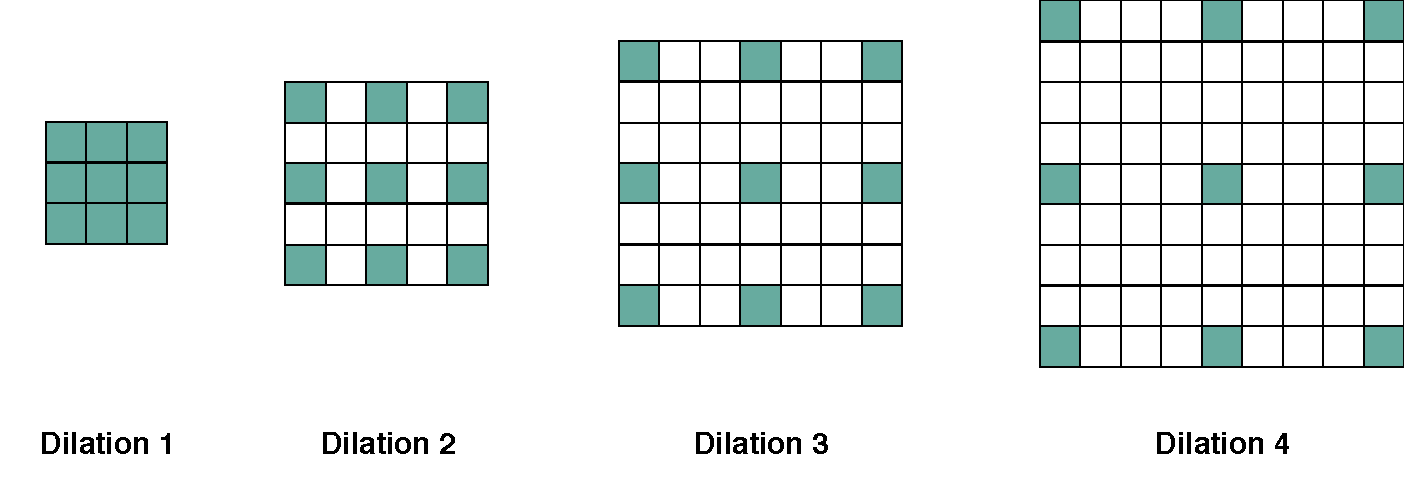
\includegraphics[width=\textwidth]{dilations.pdf}
    \caption{Kernels for dilated convolutions with successively increasing receptive field sizes.  Figure copied from \citet{antoniou2018dilated} with permission.}
    \label{fig:dilation}
\end{figure}

In this task you should investigate different approaches to modelling image context in the classification of EMNIST.  We suggest that you explore pooling, striding, and dilation, as mentioned above.  The material in the \texttt{coursework\_2} GitHub provides examples of convolutional networks, documented in \texttt{notes/pytorch-experiment-framework.md}, with code in \texttt{mlp/pytorch\_experiment\_scripts}.  The provided framework supports max and average pooling, strided convolutions and dilated convolutions.

You should thus construct, carry out, and report a set of experiments, to address one or more research questions. (An example research question might be ``does max pooling lead to more accurate classification than average pooling?''.)   

The expected amount of work for this task is a set of experiments which explore the different ways of modelling context in image classification using convolutional networks. Your experiments should involve \emph{at  most} 100h of GPU computation (using a single K80 GPU), which corresponds to the amount of computation covered by your voucher. Please note that we will not be able to provide extra credits in case the provided ones are spent.

Note that the default hyperparameters provided in the framework (see\\ \texttt{pytorch\_experiment\_scripts/experiment\_builder.py}) are reasonable -- extensive hyperparameter searches are  not required in this coursework.  As a starting point you can explore a convolutional network using 4 convolutional layers with 64 filters, which is easy to run using the script \texttt{pytorch\_experiment\_scripts/train\_evaluate\_emnist\_classification\_system.py} with the default \texttt{num\_layers} and \texttt{num\_filters} options.

Important things to note about experiments:
\begin{itemize}
    \item Your experiments should be designed so you are only varying one component at a time, so you can see the effect of that component-change.
    \item Designing experiments so that you are in a position to draw conclusions from your experiments is more important than the doing as many experiments as possible.
    \item When reporting the results of experiments, make sure that the comparison/contrast you are exploring is clear in the way you present the results.
\end{itemize}

Your report on this task should include the following:
\begin{itemize}
    \item \textbf{Introduction}.  Outline and explain the research questions you are investigating.  Provide citations if appropriate.
    \item \textbf{Methodology}.  Explain the methodology used -- in this case the approaches to modelling image context that have you explored.   Provide citations if appropriate.
    \item \textbf{Experiments}.  Describe carefully the experiments carried out, providing enough information to make them reproducible.  Present your results clearly and concisely.  Graphs and tables should be constructed to make clear the contrasts and comparisons you are interested in based on the research questions. For instance, some interesting evaluation criteria that can be used to compare different strategies are classification accuracy and speed of your network.
    \item \textbf{Discussion and conclusions.}  Discuss your results, with reference to the research questions, and if appropriate with reference to the literature.  What conclusions can you draw from your experiments?
\end{itemize}


\subsubsection*{Using Google Compute Engine}
\begin{enumerate}
    \item You will receive an email containing the URL you will need to access in order to request a Google Cloud Platform coupon, and information about how to do this.
    \item In the \texttt{coursework\_2} branch of the GitHub, \texttt{notes/google\_cloud\_setup.md} gives the instructions you should follow to set up a Google Compute Engine instance to carry out this coursework.
    \item The PyTorch experimental framework that is used for this coursework is described in\\\texttt{notes/pytorch-experiment-framework.md} and in\\\texttt{notebooks/Coursework\_2\_Pytorch\_experiment\_framework.ipynb}
\end{enumerate}

\emph{(65 Marks)}

\section{Report}
\label{sec:report}
Your coursework will be primarily assessed based on your submitted report.

The directory \verb+coursework_2/report+ contains a template for your report (\verb+mlp-cw2-template.tex+);  the generated pdf file (\verb+mlp-cw2-template.pdf+) is also provided, and you should read this file carefully as it contains some useful information about the required structure and content. The template is written in LaTeX, and we strongly recommend that you write your own report using LaTeX, using the supplied document style \verb+mlp2018+ (as in the template).

You should copy the files in the \verb+report+ directory to the directory containing the LaTeX file of your report, as \verb+pdflatex+ will need to access these files when building the pdf document from the LaTeX source file. The  \href{http://www.inf.ed.ac.uk/teaching/courses/mlp/2018-19/mlp_cw1_2018-19.pdf}{coursework 1 spec} outlines how to create a pdf file from a LaTeX source file.

Your report should be in a 2-column format, based on the document format used for the ICML conference. The report should be a \textbf{maximum of \pagelimit pages long}, not including references.  We will not read or assess any parts of the report beyond this limit.

As discussed in the \href{http://www.inf.ed.ac.uk/teaching/courses/mlp/2018-19/mlp_cw1_2018-19.pdf}{coursework 1 spec},  all figures should ideally be included in your report file as vector graphics files, rather than raster files as this will make sure all detail in the plot is visible.
% Matplotlib supports saving high quality figures in a wide range of
% common image formats using the
% \href{http://matplotlib.org/api/pyplot_api.html\#matplotlib.pyplot.savefig}{\texttt{savefig}}
% function. \textbf{You should use \texttt{savefig} rather than copying
% the screen-resolution raster images outputted in the notebook.} An
% example of using \texttt{savefig} to save a figure as a PDF file (which
% can be included as graphics in
% \href{https://en.wikibooks.org/wiki/LaTeX/Importing_Graphics}{LaTeX}
% compiled with \texttt{pdflatex} 
% %and in Apple Pages and \href{https://support.office.com/en-us/article/Add-a-PDF-to-your-Office-file-74819342-8f00-4ab4-bcbe-0f3df15ab0dc}{Microsoft Word} documents)
% is given below.

% \begin{Shaded}
% \begin{Highlighting}[]
% \CharTok{import} \NormalTok{matplotlib.pyplot }\CharTok{as} \NormalTok{plt}
% \CharTok{import} \NormalTok{numpy }\CharTok{as} \NormalTok{np}
% \CommentTok{# Generate some example data to plot}
% \NormalTok{x = np.linspace(}\DecValTok{0}\NormalTok{., }\DecValTok{1}\NormalTok{., }\DecValTok{100}\NormalTok{)}
% \NormalTok{y1 = np.sin(}\DecValTok{2}\NormalTok{. * np.pi * x)}
% \NormalTok{y2 = np.cos(}\DecValTok{2}\NormalTok{. * np.pi * x)}
% \NormalTok{fig_size = (}\DecValTok{6}\NormalTok{, }\DecValTok{3}\NormalTok{)  }\CommentTok{# Set figure size in inches (width, height)}
% \NormalTok{fig = plt.figure(figsize=fig_size)  }\CommentTok{# Create a new figure object}
% \NormalTok{ax = fig.add_subplot(}\DecValTok{1}\NormalTok{, }\DecValTok{1}\NormalTok{, }\DecValTok{1}\NormalTok{)  }\CommentTok{# Add a single axes to the figure}
% \CommentTok{# Plot lines giving each a label for the legend and setting line width to 2}
% \NormalTok{ax.plot(x, y1, linewidth=}\DecValTok{2}\NormalTok{, label=}\StringTok{'$y = \textbackslash{}sin(2\textbackslash{}pi x)$'}\NormalTok{)}
% \NormalTok{ax.plot(x, y2, linewidth=}\DecValTok{2}\NormalTok{, label=}\StringTok{'$y = \textbackslash{}cos(2\textbackslash{}pi x)$'}\NormalTok{)}
% \CommentTok{# Set the axes labels. Can use LaTeX in labels within $...$ delimiters.}
% \NormalTok{ax.set_xlabel(}\StringTok{'$x$'}\NormalTok{, fontsize=}\DecValTok{12}\NormalTok{)}
% \NormalTok{ax.set_ylabel(}\StringTok{'$y$'}\NormalTok{, fontsize=}\DecValTok{12}\NormalTok{)}
% \NormalTok{ax.grid(}\StringTok{'on'}\NormalTok{)  }\CommentTok{# Turn axes grid on}
% \NormalTok{ax.legend(loc=}\StringTok{'best'}\NormalTok{, fontsize=}\DecValTok{11}\NormalTok{)  }\CommentTok{# Add a legend}
% \NormalTok{fig.tight_layout()  }\CommentTok{# This minimises whitespace around the axes.}
% \NormalTok{fig.savefig(}\StringTok{'file-name.pdf'}\NormalTok{) }\CommentTok{# Save figure to current directory in PDF format}
% \end{Highlighting}
% \end{Shaded}


If you make use of any any books, articles, web pages or other resources
you should appropriately cite these in your report. You do not need to
cite material from the course lecture slides or lab notebooks.



% To create a pdf file \verb+mlp-cw2-template.pdf+ from a LaTeX source file (\verb+mlp-cw2-template.tex+), you can run the following in a terminal:
% \begin{verbatim}
% pdflatex mlp-cw2-template
% bibtex mlp-cw2-template
% pdflatex mlp-cw2-template
% pdflatex mlp-cw2-template
% \end{verbatim}
% (Yes, you have to run pdflatex multiple times, in order  for latex to construct the internal document references.)

% An alternative, simpler approach uses the \verb+latexmk+ program:
% \begin{verbatim}
% latexmk -pdf mlp-cw2-template
% \end{verbatim}

% Another alternative is to use an online LaTeX authoring environment such as \url{https://overleaf.com} -- note that all staff and students have free access to Overleaf Pro - see \url{https://www.ed.ac.uk/information-services/computing/desktop-personal/software/main-software-deals/other-software/overleaf}.

% It is worth learning how to use LaTeX effectively, as it is particularly powerful for mathematical and academic writing.  There are many tutorials on the web.


\section{Mechanics}
\label{sec:mechanics}

\textbf{Marks:} 
This assignment will be assessed out of 100 marks and forms \markweight\% of your final grade for the course.

\textbf{Academic conduct:} 
Assessed work is subject to University
regulations on academic
conduct:\\ {\small \url{http://web.inf.ed.ac.uk/infweb/admin/policies/academic-misconduct}}

\textbf{Submission:} 
You can submit more than once up until the submission deadline. All
submissions are timestamped automatically. Identically named files
will overwrite earlier submitted versions, so we will mark the latest
submission that comes in before the deadline.

If you submit anything before the deadline, you may not resubmit
after the deadline. (This policy allows us to begin marking submissions
immediately after the deadline, without having to worry that some may
need to be re-marked).

If you do not submit anything before the deadline, you may submit {\em
exactly once} after the deadline, and a late penalty will be applied
to this submission unless you have received an approved extension.
Please be aware that late submissions may receive lower priority for
marking, and marks may not be returned within the same timeframe as
for on-time submissions.

{\em Warning:} Unfortunately the \verb+submit+ command will technically
allow you to submit late even if you submitted before the deadline
(i.e.\ it does not enforce the above policy). Don't do this! We will
mark the version that we retrieve just after the deadline.

\textbf{Extension requests:} 
For additional information about late penalties and extension
requests, see the School web page below. \textbf{Do  not email any course
staff directly about extension requests as these are handled by the ITO; 
you must follow the instructions on the web page.}

{\small \url{http://web.inf.ed.ac.uk/infweb/student-services/ito/admin/coursework-projects/late-coursework-extension-requests}}

\textbf{Late submission penalty:}  
Following the University guidelines, 
late coursework submitted without an authorised extension will be
recorded as late and the following penalties will apply: 5
percentage points will be deducted for every calendar day or part
thereof it is late, up to a maximum of 7 calendar days. After this
time a mark of zero will be recorded.

\subsection{Backing up your work}
\label{sec:backing-up-your-work}

It is \textbf{strongly recommended} you use some method for backing up
your work. Those working in their AFS homespace on DICE will have their
work automatically backed up as part of the
\href{http://computing.help.inf.ed.ac.uk/backups-and-mirrors}{routine
backup} of all user homespaces. If you are working on a personal
computer you should have your own backup method in place (e.g.~saving
additional copies to an external drive, syncing to a cloud service or
pushing commits to your local Git repository to a private repository on
Github). \textbf{Loss of work through failure to back up
\href{http://web.inf.ed.ac.uk/infweb/student-services/ito/admin/coursework-projects/late-coursework-extension-requests}{does not constitute a good reason for
late submission}}.

You may \emph{additionally} wish to keep your coursework under version
control in your local Git repository on the \verb+coursework_2+ branch.

If you make regular commits of your work on the coursework this will
allow you to better keep track of the changes you have made and if
necessary revert to previous versions of files and/or restore
accidentally deleted work. This is not however required and you should
note that keeping your work under version control is a distinct issue
from backing up to guard against hard drive failure. If you are working
on a personal computer you should still keep an additional back up of
your work as described above.



\subsection{Submission}
\label{sec:submission}

Your coursework submission should be done electronically using the
\href{http://computing.help.inf.ed.ac.uk/submit}{\texttt{submit}}
command available on DICE machines.

Your submission should include

\begin{itemize}

\item
  your completed report as a PDF file, using the provided template
\item
  your local version of the \texttt{mlp} code including any changes
  you made to the modules (\texttt{.py} files)
 \item your personalised \texttt{test\_max\_pooling\_results\_pack.npz} and \texttt{test\_convolution\_results\_pack.npz} files. These can be automatically generated by activating your conda mlp environment and pointing your terminal to the directory \texttt{scripts} in the \texttt{mlpractical} repo and running the following commands: 
 \begin{verbatim}
python generate_conv_layer_test_file.py --student_id sXXXXXX
python generate_max_pool_layer_test_file.py --student_id sXXXXXXX
\end{verbatim}
Replace the sXXXXXXX with your student ID. Once the commands have been ran, the two .npz files will be generated under the scripts folder. You should make sure those files are included as part of your submission folder.

 \item your local version of the Pytorch experiment framework (\texttt{mlp/pytorch\_experiment\_scripts}), including any changes you've made to existing files and any newly created files.
 \item a copy of your Pytorch experiment directories, including \textbf{only} the \texttt{.csv} files for your training, validation and test statistics. Please do not include model weights.

\end{itemize}
Please do not submit anything else (e.g. log files).

You should copy all of the files to a single directory, \verb+coursework2+, e.g.

\begin{verbatim}
mkdir coursework2
cp reports/coursework2.pdf coursework2
cp scripts/test_max_pooling_results_pack.npz  coursework2
cp scripts/test_convolution_results_pack.npz  coursework2
\end{verbatim}
also copy to \texttt{coursework2} the directories containing your mlp and PyTorch code, as well as the directory containing the PyTorch \texttt{csv} files.
%cp sXXXXXXX_batchnorm_test_file.txt sXXXXXXX_conv_test_file.txt 


You should then submit this directory using

\begin{verbatim}
submit mlp cw2 coursework2
\end{verbatim}

\textbf{Please submit the directory, not a zip file, not a tar file.}

The \texttt{submit} command will prompt you with the details of the
submission including the name of the files / directories you are
submitting and the name of the course and exercise you are submitting
for and ask you to check if these details are correct. You should check
these carefully and reply \texttt{y} to submit if you are sure the files
are correct and \texttt{n} otherwise.

You can amend an existing submission by rerunning the \texttt{submit}
command any time up to the deadline. It is therefore a good idea
(particularly if this is your first time using the DICE submit
mechanism) to do an initial run of the \texttt{submit} command early on
and then rerun the command if you make any further updates to your
submission rather than leaving submission to the last minute.


\section{Marking Guidelines}
\label{sec:marking-scheme}
This document (Section \ref{sec:tasks} in particular) and the template report (\verb+mlp-cw1-template.pdf+) provide a description of what you are expected to do in this assignment, and how the report should be written and structured.

Assignments will be marked using the scale defined by the \textbf{University Common Marking Scheme}:
\begin{center}
\begin{tabular}{lll}
Numeric mark & Equivalent letter grade & Approximate meaning \\
$< 40$ & F & fail \\
40-49 & D & poor \\
50-59 & C & acceptable \\
60-69 & B & good \\
70-79 & A3 & very good/distinction \\
80-100 & A1, A2 & excellent/outstanding/high distinction
\end{tabular}
\end{center}

Please note the University specifications for marks above 70:

{\bf A1 90-100}
Often faultless. The work is well beyond what is expected for the level of study.

{\bf A2 80-89}
A truly professional piece of scholarship, often with an absence of errors. \\
As `A3' but shows (depending upon the item of assessment):
significant personal insight / creativity / originality
and / or
extra depth and academic maturity in the elements of assessment.

{\bf A3 70-79}\\
\emph{Knowledge}: Comprehensive range of up-to-date material handled in a professional way.\\
\emph{Understanding/handling of key concepts}: Shows a command of the subject and current theory.\\
\emph{Focus on the subject}: Clear and analytical; fully explores the subject.\\
\emph{Critical analysis and discussion}: Shows evidence of serious thought in critically evaluating and integrating the evidenced and ideas. Deals confidently with the complexities and subtleties of the arguments. Shows elements of personal insight / creativity / originality.\\
\emph{Structure}: Clear and coherent showing logical, ordered thought.\\
\emph{Presentation}: Clear and professional with few, relatively minor flaws. Accurate referencing. Figures and tables well constructed and accurate. Good standard of spelling and grammar.
\bibliographystyle{plainnat}
\bibliography{mlp-cw-references}
\end{document}
